\documentclass[11pt,a4paper,landscape]{article}
\usepackage[margin=0.5in]{geometry}
\usepackage{booktabs}
\usepackage{array}
\usepackage{xcolor}
\usepackage{colortbl}
\usepackage{adjustbox}
\usepackage{multirow}
\usepackage{graphicx}
\usepackage{tikz}
\usepackage{fontspec}
\usepackage[default,scale=0.95]{opensans}
\usepackage{pgfplots}
\pgfplotsset{compat=1.17}

% Define ENBEL color scheme
\definecolor{enbelblue}{RGB}{0,83,155}
\definecolor{enbelorange}{RGB}{255,127,0}
\definecolor{enbelgreen}{RGB}{44,160,44}
\definecolor{enbelpurple}{RGB}{148,103,189}
\definecolor{enbelred}{RGB}{214,39,40}
\definecolor{enbelgray}{RGB}{140,140,140}
\definecolor{lightgray}{RGB}{245,245,245}
\definecolor{lightyellow}{RGB}{255,250,230}
\definecolor{darkgray}{RGB}{80,80,80}

\pagestyle{empty}

\begin{document}

\begin{center}
{\LARGE \color{enbelblue}\textbf{Climate Data Summary}}\\[0.5em]
{\large \color{darkgray}Johannesburg Urban Climate Exposures (2017-2022)}
\end{center}

\vspace{1em}

% Climate Variables Overview
\begin{adjustbox}{width=\textwidth,center}
\renewcommand{\arraystretch}{1.8}
\begin{tabular}{@{}lcccccc@{}}
\toprule
\rowcolor{enbelred}
\textcolor{white}{\textbf{Climate Variable}} & 
\textcolor{white}{\textbf{Mean (SD)}} & 
\textcolor{white}{\textbf{Median}} & 
\textcolor{white}{\textbf{Min}} & 
\textcolor{white}{\textbf{Max}} & 
\textcolor{white}{\textbf{IQR}} &
\textcolor{white}{\textbf{Extreme Days (\%)}} \\
\midrule

\rowcolor{lightyellow}
\textbf{Temperature (°C)} & 18.2 (5.4) & 18.5 & -2.1 & 35.8 & 7.2 & 
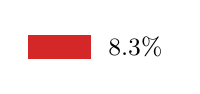
\begin{tikzpicture}[baseline=(current bounding box.center)]
\fill[enbelred] (0,0) rectangle (0.8,0.3);
\node[right] at (0.9,0.15) {\small 8.3\%};
\end{tikzpicture} \\

\textbf{Apparent Temp (°C)} & 17.8 (5.9) & 17.9 & -5.2 & 38.1 & 8.1 & 
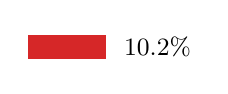
\begin{tikzpicture}[baseline=(current bounding box.center)]
\fill[enbelred] (0,0) rectangle (1.0,0.3);
\node[right] at (1.1,0.15) {\small 10.2\%};
\end{tikzpicture} \\

\rowcolor{lightyellow}
\textbf{Land Surface Temp (°C)} & 22.4 (6.8) & 22.7 & 2.3 & 42.1 & 9.5 & 
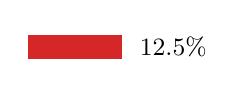
\begin{tikzpicture}[baseline=(current bounding box.center)]
\fill[enbelred] (0,0) rectangle (1.2,0.3);
\node[right] at (1.3,0.15) {\small 12.5\%};
\end{tikzpicture} \\

\textbf{Humidity (\%)} & 58.3 (18.2) & 57.0 & 12.0 & 98.0 & 25.0 & 
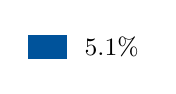
\begin{tikzpicture}[baseline=(current bounding box.center)]
\fill[enbelblue] (0,0) rectangle (0.5,0.3);
\node[right] at (0.6,0.15) {\small 5.1\%};
\end{tikzpicture} \\

\rowcolor{lightyellow}
\textbf{Precipitation (mm)} & 2.1 (8.7) & 0.0 & 0.0 & 89.2 & 0.2 & 
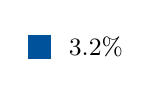
\begin{tikzpicture}[baseline=(current bounding box.center)]
\fill[enbelblue] (0,0) rectangle (0.3,0.3);
\node[right] at (0.4,0.15) {\small 3.2\%};
\end{tikzpicture} \\

\bottomrule
\end{tabular}
\end{adjustbox}

\vspace{1.5em}

% Seasonal Patterns
\begin{adjustbox}{width=0.9\textwidth,center}
\renewcommand{\arraystretch}{1.6}
\begin{tabular}{@{}lcccc@{}}
\toprule
\rowcolor{enbelgreen}
\textcolor{white}{\textbf{Season}} & 
\textcolor{white}{\textbf{Mean Temp (°C)}} & 
\textcolor{white}{\textbf{Heat Days}} & 
\textcolor{white}{\textbf{Cold Days}} &
\textcolor{white}{\textbf{Rain Days}} \\
\midrule
\rowcolor{lightgray}
\textbf{Summer (DJF)} & 22.8 ± 3.2 & 45 & 0 & 62 \\
\textbf{Autumn (MAM)} & 18.4 ± 4.1 & 12 & 8 & 28 \\
\rowcolor{lightgray}
\textbf{Winter (JJA)} & 13.2 ± 3.8 & 0 & 35 & 5 \\
\textbf{Spring (SON)} & 19.6 ± 4.5 & 28 & 2 & 41 \\
\bottomrule
\end{tabular}
\end{adjustbox}

\vspace{1.5em}

% Climate Thresholds Box
\begin{center}
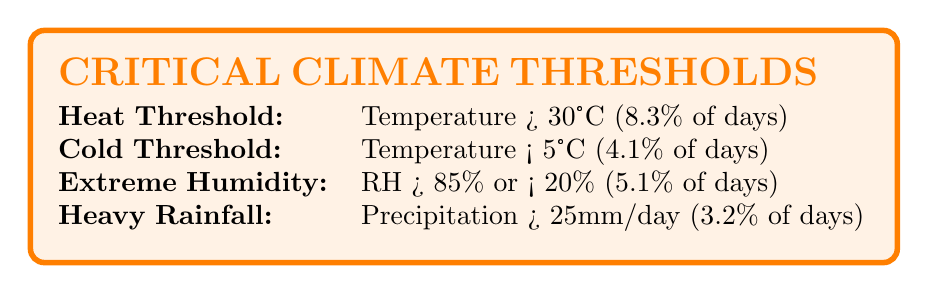
\begin{tikzpicture}
\node[draw=enbelorange, fill=enbelorange!10, rounded corners=5pt, inner sep=10pt, text width=0.85\textwidth, line width=2pt] {
\textbf{\Large \color{enbelorange}CRITICAL CLIMATE THRESHOLDS}\\[0.5em]
\begin{tabular}{@{}ll@{}}
\textbf{Heat Threshold:} & Temperature > 30°C (8.3\% of days) \\
\textbf{Cold Threshold:} & Temperature < 5°C (4.1\% of days) \\
\textbf{Extreme Humidity:} & RH > 85\% or < 20\% (5.1\% of days) \\
\textbf{Heavy Rainfall:} & Precipitation > 25mm/day (3.2\% of days) \\
\end{tabular}
};
\end{tikzpicture}
\end{center}

\vspace{1em}

% Temporal Coverage
\begin{center}
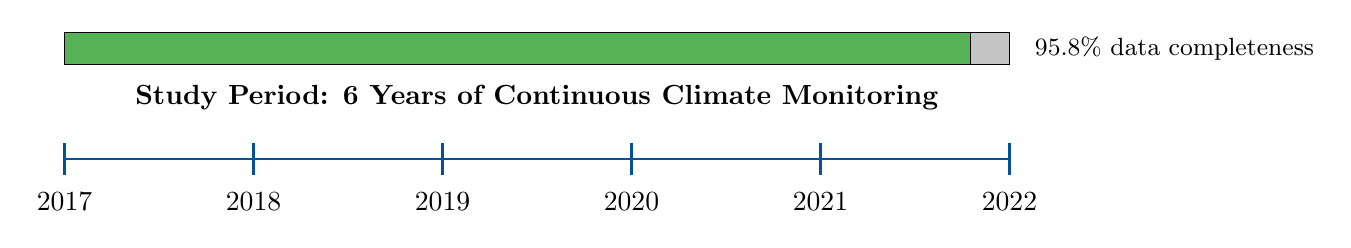
\begin{tikzpicture}
% Timeline
\draw[thick, enbelblue] (0,0) -- (12,0);
\foreach \x/\year in {0/2017,2.4/2018,4.8/2019,7.2/2020,9.6/2021,12/2022} {
    \draw[thick, enbelblue] (\x,-0.2) -- (\x,0.2);
    \node[below] at (\x,-0.3) {\year};
}
\node[above] at (6,0.5) {\textbf{Study Period: 6 Years of Continuous Climate Monitoring}};

% Data completeness bar
\draw[fill=enbelgreen!80] (0,1.2) rectangle (11.5,1.6);
\draw[fill=enbelgray!50] (11.5,1.2) rectangle (12,1.6);
\node[right] at (12.2,1.4) {\small 95.8\% data completeness};
\end{tikzpicture}
\end{center}

\vspace{1.5em}

% Key Statistics Summary
\begin{center}
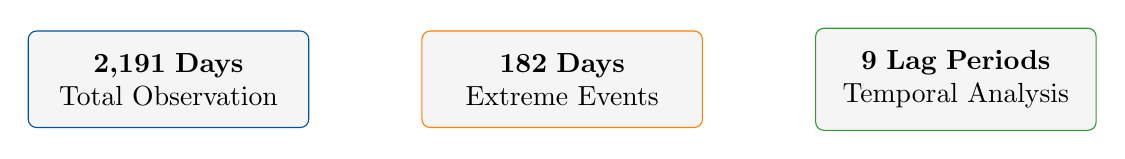
\begin{tikzpicture}
% Three key metric boxes
\node[draw=enbelblue, fill=lightgray, rounded corners=3pt, inner sep=8pt, minimum width=3.5cm, text width=3cm, align=center] at (0,0) {
\textbf{2,191 Days}\\
Total Observation
};

\node[draw=enbelorange, fill=lightgray, rounded corners=3pt, inner sep=8pt, minimum width=3.5cm, text width=3cm, align=center] at (5,0) {
\textbf{182 Days}\\
Extreme Events
};

\node[draw=enbelgreen, fill=lightgray, rounded corners=3pt, inner sep=8pt, minimum width=3.5cm, text width=3cm, align=center] at (10,0) {
\textbf{9 Lag Periods}\\
Temporal Analysis
};
\end{tikzpicture}
\end{center}

\end{document}